\chapter{Исследовательская часть}
\hspace{\parindent}В данном разделе будет проведен сравнительный анализ алгоритмов по времени выполнения в зависимости от количества матриц и их размеров.

\section{Технические характеристики}
\hspace{\parindent}Технические характеристики устройства, на котором выполнялось тестирование представлены далее:

\begin{enumerate}
    \item операционная система: Windows 10 pro;
    \item память: 32 Гб;
    \item процессор: 12h Gen Intel(R) Core(TM) i5-12400 2.50 Ггц.
\end{enumerate}
\hspace{\parindent}Во время замеров компьютер был включен в сеть электропитания и был нагружен только системными программами и программой замеров.
\clearpage

\section{Демонстрация работы программы}
\hspace{\parindent}На рис. \ref{fig:demonstration} представлена демонстрация работы программы. 

\begin{figure}[h]
	\centering
	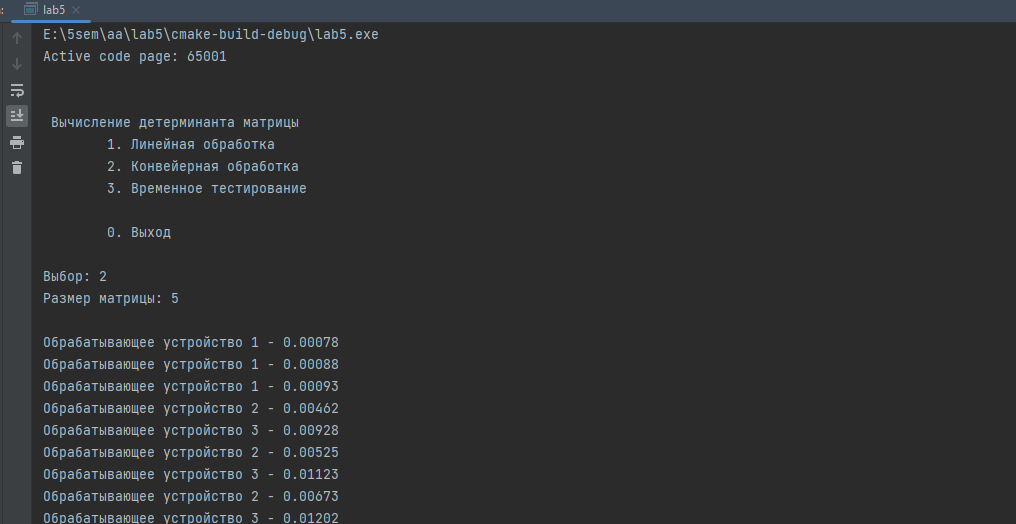
\includegraphics[height=0.5\textheight]{img/ex.png}
	\caption{Демонстрация работы программы}
	\label{fig:demonstration}
\end{figure}

\clearpage
\section{Время выполнения алгоритмов}
\hspace{\parindent}Результаты замеров приведены в таблицах \ref{tbl:time1}-\ref{tbl:time4}. Время указано в секундах.

\begin{table}[h]
    \begin{center}
    	\centering
    	\captionsetup{skip=0pt,justification=raggedright,singlelinecheck=off}
        \caption{Результаты замеров по времени для матриц размером 7}
        \label{tbl:time1}
        \begin{tabular}{|r|r|r|}
            \hline
            Количество матриц & Линейная & Конвейерная\\
           \hline
           1 & 0.0109 & 0.0118 \\
           \hline
           2 & 0.0223 & 0.0231 \\
           \hline
           3 & 0.0294 & 0.0331 \\
           \hline
           4 & 0.0430 & 0.0378 \\
           \hline
		\end{tabular}
	\end{center}
\end{table}
\begin{table}[h]
	\begin{center}
		\centering
		\captionsetup{skip=0pt,justification=raggedright,singlelinecheck=off}
		\caption{Результаты замеров по времени для матриц размером 8}
		\label{tbl:time2}
		\begin{tabular}{|r|r|r|}
			\hline
			Количество матриц & Линейная & Конвейерная\\
			\hline
			1 & 0.0815 & 0.0495 \\
			\hline
			2 & 0.1555 & 0.0940 \\
			\hline
			3 & 0.2385 & 0.1402 \\
			\hline
			4 & 0.3259 & 0.1944 \\
			\hline
		\end{tabular}
	\end{center}
\end{table}
\begin{table}[h]
	\begin{center}
		\centering
		\captionsetup{skip=0pt,justification=raggedright,singlelinecheck=off}
		\caption{Результаты замеров по времени для матриц размером 9}
		\label{tbl:time3}
		\begin{tabular}{|r|r|r|}
			\hline
			Количество матриц & Линейная & Конвейерная\\
			\hline
			1 & 0.7050 & 0.4097 \\
			\hline
			2 & 1.4126 & 0.8191 \\
			\hline
			3 & 2.1326 & 1.2208 \\
			\hline
			4 & 2.8180 & 1.5875 \\
			\hline
		\end{tabular}
	\end{center}
\end{table}
\begin{table}[H]
	\begin{center}
		\centering
		\captionsetup{skip=0pt,justification=raggedright,singlelinecheck=off}
		\caption{Результаты замеров по времени для матриц размером 10}
		\label{tbl:time4}
		\begin{tabular}{|r|r|r|}
			\hline
			Количество матриц & Линейная & Конвейерная\\
			\hline
			1 & 7.0369 & 3.6058 \\
			\hline
			2 & 14.1037 & 7.1952 \\
			\hline
			3 & 21.2308 & 10.6358 \\
			\hline
			4 & 28.1996 & 14.8571 \\
			\hline
		\end{tabular}
	\end{center}
\end{table}